\documentclass[thesis.tex]{subfiles}

\begin{document}
Once the ground state energy and the effective Hamiltonian has been calculated, any further properties of the ground state can be calculated using the correlated wave function written as a Slater determinant expansion in the form of Eqn.\ \cite{eq:cc_ansatz}.  However, many of the most interesting processes in nuclear physics involve excited-state properties.  Additionally, because the coupled cluster method requires a doubly closed-shell reference state, most topics in nuclear phyics that can benefit from an ab initio description are unreachable with the standard coupled cluster approach alone.

These restrictions motivates a class of techniques known as \texit{equations-of-motion} methods (EOM).  Applied with the CC effective Hamiltonian, the \textit{coupled-cluster equations-of-motion} CC-EOM method begins with a standard CC calculation of a closed-shell ground state.  Then, EOM \texit{target states} are built onto the correlated ground-state wave function in the same way that CI states were built from the reference state, Eqn.\ \cite{eq:ci_expansion}.  Unfortunately, because the CCSD similarity transformation only decouples the ground state from $\ph{1}{1}$ and $\ph{2}{2}$ excitations, these target states are still coupled to each other.  Therefore, capturing the relevant correlations to describe EOM states involves a CI-like diagonalization of the effective Hamiltonian.


\section{Equations-of-Motion States} \label{section:eom_target_states}

The CC equations-of-motion states are built by applying a particular type of excitation operator to the correlated ground-state wave function.
\begin{equation}\label{eq:ladder_def}
  \ket{\Psi_{\mu}} = \Rop_{\mu}\corrket = \Rop_{\mu}\E^{\Top}\refket,
\end{equation}
where $\Rop_{\mu}$ can be written as a linear combination of strings of creation and annihilation operators.  The form of these strings is determined by the structure of the desired target state.  For example, excited states maintain the particle number of the reference state and ground state so that the constiuent operator strings are $\ph{k}{k}$ operators.  The $A$-particle excited-state EOM operator $\Rop^{A}_{\mu}$ is,
\begin{equation}
  \Rop^{A}_{\mu} = \rint{\mu}{}{0} + \sum_{ai}\rint{\mu}{a}{i}\normord{\co{a}\ao{i}} + \frac{1}{4}\sum_{abij}\rint{\mu}{ab}{ij}\normord{\co{a}\co{b}\ao{j}\ao{i}} + \cdots
\end{equation}
Particle attached and particle removed equations-of-motion (EOM) methods can be coupled with either IM-SRG or CC calculations. The principal idea is that one may construct a ladder operator $\hat{X}$ that promotes the $N$-particle ground state to any state in the $N + 1$ or $N - 1$ spectrum,


\begin{equation}
  \Rop^{A+1}_{\mu} = \sum_{a}\rint{\mu}{a}{}\normord{\co{a}} + \frac{1}{2}\sum_{abi}\rint{\mu}{ab}{i}\normord{\co{a}\co{b}\ao{i}} + \cdots
\end{equation}

\begin{equation}
  \Rop^{A-1}_{\mu} = \sum_{i}\rint{\mu}{}{i}\normord{\ao{i}} + \frac{1}{2}\sum_{aij}\rint{\mu}{a}{ij}\normord{\co{a}\ao{j}\ao{i}} + \cdots
\end{equation}

\begin{equation}
  \Lop^{A+1}_{\mu} = \sum_{a}\lint{\mu}{}{a}\normord{\ao{a}} + \frac{1}{2}\sum_{abi}\lint{\mu}{i}{ab}\normord{\co{i}\ao{b}\ao{}} + \cdots
\end{equation}

\begin{equation}
  \Lop^{A-1}_{\mu} = \sum_{i}\lint{\mu}{i}{}\normord{\co{i}} + \frac{1}{2}\sum_{aij}\lint{\mu}{ij}{a}\normord{\co{i}\co{j}\ao{a}} + \cdots
\end{equation}

\begin{equation}
  \braket{\Lop_{\mu}}{\Rop_{\nu}} = \delta_{\mu\nu}
\end{equation}

Here, $\rint{\mu}{}{}$ are the normal-ordered matrix elements of $\Rop_{\mu}$.

Substitution of Eq.\ \eqref{eq:ladder_def} into the energy eigenvalue problem
\begin{equation}
  \Ham\ket{\Psi_{\mu}} = E_{\mu}\ket{\Psi_{\mu}},
\end{equation}
\begin{gather}
  \HamN\ket{\Psi_{\mu}} = \Ecorr_{\mu}\ket{\Psi_{\mu}} \notag \\
  \HamN\Rop_{\mu}\E^{\Top}\refket = \Ecorr_{\mu}\Rop_{\mu}\E^{\Top}\refket \notag \\
  \E^{-\Top}\HamN\Rop_{\mu}\E^{\Top}\refket = \E^{-\Top}\Ecorr_{\mu}\Rop_{\mu}\E^{\Top}\refket
\end{gather}
\begin{gather}
  \E^{-\Top}\HamN\E^{\Top}\Rop_{\mu}\refket = \Ecorr_{\mu}\E^{-\Top}\E^{\Top}\Rop_{\mu}\refket \notag \\
  \EHamN\Rop_{\mu}\refket = \Ecorr_{\mu}\Rop_{\mu}\refket
\end{gather}
\begin{align}
  \EHamN\Rop_{\mu}\refket &= \Ecorr_{\mu}\Rop_{\mu}\refket \notag \\
  -\Rop_{\mu}\EHamN\refket &= \Rop_{\mu}\Ecorr\refket \notag \\
  \longrightarrow\ \ [\EHamN,\Rop_{\mu}]\refket &= (\Ecorr_{\mu} - \Ecorr)\Rop_{\mu}\refket = \omega_{\mu}\Rop_{\mu}\refket
\end{align}


\begin{equation}\label{eq:ladder_def}
  \bra{\Psi_{\mu}} = \refbra\Lop_{\mu}
\end{equation}
\begin{gather}
  \bra{\Psi_{\mu}}\EHamN = \bra{\Psi_{\mu}}\Ecorr_{\mu} \notag \\
  \refbra\Lop_{\mu}\EHamN = \refbra\Lop_{\mu}\Ecorr_{\mu},
\end{gather}


\begin{gather}
  [\EHamN,\Rop_{\mu}] = \omega_{\mu}\Rop_{\mu} \notag \\
  \Lop_{\mu}\EHamN = \Lop_{\mu}\Ecorr_{\mu}
\end{gather}


gives
\begin{equation}\label{eq:EOM}
  [\Ham, \Rop_{\mu}] \corrket = \pm \varepsilon^{(\pm)}_u \hat{X}^{(N \pm 1)}_u \ket{\Psi^{(N)}_0},
\end{equation}
which constitutes a generalized eigenvalue problem for the amplitudes $x$, where $\varepsilon^{(\pm)}_u$ are the single-particle addition ($+$) and removal ($-$) energies. The quality of this calculation depends on the ansatz for the $N$-particle ground state, as well as the systematically improvable truncation on the ladder operators. In this work we include 1p and 2p1h excitations in the $N + 1$ ladder operator and likewise 1h and 2h1p operators for the $N - 1$ ladder operators.

After a single-reference ground state IM-SRG calculation, the Hamiltonian has been rotated such that the reference state is an eigenfunction with corresponding eigenvalue $E^{(N)}_0$, which is the correlated $N$-particle ground state energy. The EOM equation is therefore
\begin{align} \label{eq:EOMIMSRG}
  [\bar{H},\bar{X}^{(N \pm 1)}_u] \ket{\Phi^{(N)}_0} = \pm \varepsilon^{(\pm)}_u \bar{X}^{(N \pm 1)}_u \ket{\Phi^{(N)}_0},
\end{align}
where bars denote rotated operators. Now the reference state is used in place of the bare correlated ground state. The ground state IM-SRG procedure has implicitly re-summed contributions from higher order excitations (3-particle-2-hole, 2-particle-3-hole, 2-particle-3-hole, 4-particle-3-hole, \ldots) into the lower order amplitudes of the ladder operators (1-particle-0-hole, 0-particle-1-hole, 2-particle-1-hole, 1-particle-2-hole).

Despite these gains, the EOM calculation is still a partial diagonalization method, limited by the truncation to 2-particle-1-hole and 1-particle-2-hole operators. We expect $N + 1$ (or $N - 1$) states to be described appropriately by EOM-IM-SRG if their wavefunctions are dominated by 1-particle-0-hole (or 0-particle-1-hole) contributions in the rotated frame. We use partial norms of the EOM ladder operators to estimate these contributions:
\begin{align}
  \label{eq:partial_norms_p}
  n_{\text{1-particle}} &= \sqrt{\sum_a | \rint{\mu}{a}{} |^2},\\
  \label{eq:partial_norms_h}
  n_{\text{1-hole}} &= \sqrt{\sum_i | \rint{\mu}{a}{} |^2}.
\end{align}
Large single particle partial norms indicate that the EOM truncation is reasonable for the relevant state. States with lower single particle norms should be treated with a higher EOM approximation, which can be accomplished directly or perturbatively \cite{PARZUCHOWSKI2017044304}.

Like EOM-IM-SRG, the equations-of-motion technique can be applied after a CC ground-state calculation, by using the CC effective Hamiltonian.  Here, the non-Hermitian nature of $\bar{H}_{\mathrm{CC}}$ becomes apparent.  In this case, in addition to constructing excitation ladder operators Eq.\ \eqref{eq:gen_attached} and Eq.\ \eqref{eq:gen_removed} that correspond to the right-eigenvectors of the generalized eigenvalue problem Eq.\ \eqref{eq:EOMIMSRG}, there exist analogous de-excitation ladder operators, $\hat{L}^{(N + 1)}$ and $\hat{L}^{(N - 1)}$, that correspond to the left-eigenvectors,
\begin{align*}
    \hat{L}^{(N + 1)}_u &= \sum_a l^{(u, +)}_a \normord{\hat{a}_a^{}} + \frac{1}{2} \sum_{i a b} l^{(u, +)}_{i a b} \normord{\hat{a}^\dagger_i \hat{a}_b^{} \hat{a}_a^{}} + \cdots, \\
    \hat{L}^{(N - 1)}_u &= \sum_i l_i^{(u, -)} \normord{\hat{a}^\dagger_i} + \frac{1}{2} \sum_{i j a} l^{(u, -)}_{i j a} \normord{\hat{a}^\dagger_i \hat{a}^\dagger_j \hat{a}_a^{}} + \cdots,
\end{align*}
where $l^{(u, \pm)}_p$ and $l^{(u, \pm)}_{p q r}$ are likewise the normal-ordered matrix elements of $\hat{L}^{(N \pm 1)}_u$.  These left-eigenvectors satisfy the left-eigenvalue problem, with left-eigenvalues $\varepsilon^{(\pm)}_u$, analogous to Eq.\ \eqref{eq:EOMIMSRG},
\begin{align*}
  \bra{\Phi^{(N)}_0} [\bar{H}, \bar{L}^{(N \pm 1)}_u] = \pm \varepsilon^{(\pm)}_u \bra{\Phi^{(N)}_0} \bar{L}^{(N \pm 1)}_u
\end{align*}
and form a bi-orthogonal set with the right-eigenvectors, $\braket{\bar{L}^{(N \pm 1)}_u}{\bar{X}^{(N \pm 1)}_v} = \delta_{u v}$.

In this paper, because the effective Hamiltonian is real, the corresponding left- and right-eigenvalues are equal. In addition, while the the left- and right-eigenvectors are generally not equivalent, the differences in their single-particle Eq.\ \eqref{eq:partial_norms_p} or single-hole Eq.\ \eqref{eq:partial_norms_h} natures are, in practice, not significant.  Therefore, only the right-eigenvectors are used in this paper.


%\begin{align}
%  \langle\Phi_{0}|\hat{L}^{+1}_{\nu}\bar{H}_{N}\hat{R}^{+1}_{\nu}|\Phi_{0}\rangle_{c} &= \diagram{PA_EOM/PA_EOM-figure0} + \diagram{PA_EOM/PA_EOM-figure1} + \diagram{PA_EOM/PA_EOM-figure2} + \diagram{PA_EOM/PA_EOM-figure3} \notag \\
%  &\hspace{-2cm} + \diagram{PA_EOM/PA_EOM-figure4} + \diagram{PA_EOM/PA_EOM-figure5} + \diagram{PA_EOM/PA_EOM-figure6} + \diagram{PA_EOM/PA_EOM-figure7} \notag \\
%\end{align}

%\begin{align}
%  \langle\Phi_{0}|\hat{L}^{-1}_{\nu}\bar{H}_{N}\hat{R}^{-1}_{\nu}|\Phi_{0}\rangle_{c}\ &= \diagram{PR_EOM/PR_EOM-figure0} + \diagram{PR_EOM/PR_EOM-figure1} + \diagram{PR_EOM/PR_EOM-figure2} + \diagram{PR_EOM/PR_EOM-figure3} \notag \\
%  &\hspace{-2cm} + \diagram{PR_EOM/PR_EOM-figure4} + \diagram{PR_EOM/PR_EOM-figure5} + \diagram{PR_EOM/PR_EOM-figure6} + \diagram{PR_EOM/PR_EOM-figure7} \notag \\
%\end{align}


\begin{align} \label{eq:threebody1}
  \diagram{CCSD_3b/CCSD_3b-figure0} &= \diagram{CCSD_3b/CCSD_3b-figure1} \notag \\
  \xint{iab}{jcd} &= -\sum\limits_{k}\vint{jk}{cd}\tamp{ab}{ki}
\end{align}

\begin{align} \label{eq:threebody2}
  \diagram{CCSD_3b/CCSD_3b-figure2} &= \diagram{CCSD_3b/CCSD_3b-figure3} \notag \\
  \xint{kla}{ijb} &= \sum\limits_{k}\vint{jk}{cd}\tamp{ab}{ki}
\end{align}



\begin{align}
  \diagram{PA_EOM1/PA_EOM1-figure0} &= \diagram{PA_EOM1/PA_EOM1-figure1} + \diagram{PA_EOM1/PA_EOM1-figure2} + \diagram{PA_EOM1/PA_EOM1-figure3} \notag \\
  \omega_{k}\rop{a}{} &= \sum\limits_{c}\xint{a}{c}\rop{c}{} + \sum\limits_{kc}\xint{k}{c}\rop{ac}{k} + \frac{1}{2}\sum\limits_{kcd}\xint{ak}{cd}\rop{cd}{k}
\end{align}
\begin{align}
  \diagram{PA_EOM1/PA_EOM1-figure4} &= \diagram{PA_EOM1/PA_EOM1-figure5} + \diagram{PA_EOM1/PA_EOM1-figure6} + \diagram{PA_EOM1/PA_EOM1-figure7} + \diagram{PA_EOM1/PA_EOM1-figure8} \notag \\
  &+ \diagram{PA_EOM1/PA_EOM1-figure9} + \diagram{PA_EOM1/PA_EOM1-figure10} \notag \\
  \omega_{k}\rop{ab}{i} &= \sum\limits_{c}\xint{ab}{ci}\rop{c}{} + \Perm{ab}\sum\limits_{c}\xint{b}{c}\rop{ac}{i} - \sum\limits_{k}\xint{k}{i}\rop{ab}{k} + \frac{1}{2}\sum\limits_{cd}\xint{ab}{cd}\rop{cd}{i} \notag \\
  &-\Perm{ab}\sum\limits_{kc}\xint{ak}{ci}\rop{cb}{k} - \frac{1}{2}\sum\limits_{klcd}\vint{kl}{cd}\amp{ab}{ki}\rop{cd}{l}
\end{align}

\begin{align}
  \diagram{PA_EOM1/PA_EOM1-figure11} &= \diagram{PA_EOM1/PA_EOM1-figure12} + \diagram{PA_EOM1/PA_EOM1-figure13} \notag \\
  E_{k}\lop{}{a} &= \sum\limits_{c}\lop{}{c}\xint{c}{a} + \frac{1}{2}\sum\limits_{kcd}\lop{k}{cd}\xint{cd}{ak}
\end{align}
\begin{align}
  \diagram{PA_EOM1/PA_EOM1-figure14} &= \diagram{PA_EOM1/PA_EOM1-figure15} + \diagram{PA_EOM1/PA_EOM1-figure16} + \diagram{PA_EOM1/PA_EOM1-figure17} + \diagram{PA_EOM1/PA_EOM1-figure18} \notag \\
  &+ \diagram{PA_EOM1/PA_EOM1-figure19} + \diagram{PA_EOM1/PA_EOM1-figure20} + \diagram{PA_EOM1/PA_EOM1-figure21} \notag \\
  E_{k}\lop{i}{ab} &= \Perm{ab}\lop{}{a}\xint{i}{b} + \sum\limits_{c}\lop{}{c}\xint{ci}{ab} - \sum\limits_{k}\lop{k}{ab}\xint{i}{k} + \Perm{ab}\sum\limits_{c}\lop{i}{ac}\xint{c}{b} \notag \\
  &+ \frac{1}{2}\sum\limits_{cd}\lop{i}{cd}\xint{cd}{ab} - \Perm{ab}\sum\limits_{kc}\lop{k}{cb}\xint{ci}{ak} - \frac{1}{2}\sum\limits_{klcd}\lop{l}{cd}\vint{ki}{ab}\amp{cd}{kl}
\end{align}


\begin{align}
  \diagram{PR_EOM1/PR_EOM1-figure0} &= \diagram{PR_EOM1/PR_EOM1-figure1} + \diagram{PR_EOM1/PR_EOM1-figure2} + \diagram{PR_EOM1/PR_EOM1-figure3} \notag \\
  \omega_{k}\rop{}{i} &= -\sum\limits_{k}\xint{k}{i}\rop{}{k} + \sum\limits_{kc}\xint{k}{c}\rop{c}{ik} - \frac{1}{2}\sum\limits_{klc}\xint{kl}{ic}\rop{c}{kl}
\end{align}
\begin{align}
  \diagram{PR_EOM1/PR_EOM1-figure4} &= \diagram{PR_EOM1/PR_EOM1-figure5} + \diagram{PR_EOM1/PR_EOM1-figure6} + \diagram{PR_EOM1/PR_EOM1-figure7} + \diagram{PR_EOM1/PR_EOM1-figure8} \notag \\
  &+ \diagram{PR_EOM1/PR_EOM1-figure9} + \diagram{PR_EOM1/PR_EOM1-figure10} \notag \\
  \omega_{k}\rop{a}{ij} &= -\sum\limits_{k}\xint{ka}{ij}\rop{}{k} - \Perm{ij}\sum\limits_{k}\xint{k}{j}\rop{a}{ik} + \sum\limits_{c}\xint{a}{c}\rop{c}{ij} + \frac{1}{2}\sum\limits_{kl}\xint{kl}{ij}\rop{a}{kl} \notag \\
  &-\Perm{ij}\sum\limits_{kc}\xint{ak}{ci}\rop{c}{kj} - \frac{1}{2}\sum\limits_{klcd}\vint{kl}{cd}\amp{ca}{ij}\rop{d}{kl}
\end{align}

\begin{align}
  \diagram{PR_EOM1/PR_EOM1-figure11} &= \diagram{PR_EOM1/PR_EOM1-figure12} + \diagram{PR_EOM1/PR_EOM1-figure13} \notag \\
  E_{k}\lop{i}{} &= -\sum\limits_{k}\lop{k}{}\xint{i}{k} - \frac{1}{2}\sum\limits_{klc}\lop{kl}{c}\xint{ic}{kl}
\end{align}
\begin{align}
  \diagram{PR_EOM1/PR_EOM1-figure14} &= \diagram{PR_EOM1/PR_EOM1-figure15} + \diagram{PR_EOM1/PR_EOM1-figure16} + \diagram{PR_EOM1/PR_EOM1-figure17} + \diagram{PR_EOM1/PR_EOM1-figure18} \notag \\
  &+ \diagram{PR_EOM1/PR_EOM1-figure19} + \diagram{PR_EOM1/PR_EOM1-figure20} + \diagram{PR_EOM1/PR_EOM1-figure21} \notag \\
  E_{k}\lop{ij}{a} &= \Perm{ij}\lop{i}{}\xint{j}{a} - \sum\limits_{k}\lop{k}{}\xint{ij}{ka} + \sum\limits_{c}\lop{ij}{c}\xint{c}{a} - \Perm{ij}\sum\limits_{k}\lop{ik}{a}\xint{j}{k} \notag \\
  &+ \frac{1}{2}\sum\limits_{cd}\lop{kl}{a}\xint{ij}{kl} - \Perm{ij}\sum\limits_{kc}\lop{kj}{c}\xint{ci}{ak} - \frac{1}{2}\sum\limits_{klcd}\lop{kl}{d}\vint{ij}{ca}\amp{cd}{kl}
\end{align}


\section{EOM Results for 2D Quantum Dots} \label{section:eom_target_states}
To examine some properties of the CC-EOM method, it's useful to focus on the results from the two-dimensional quantum dot.  This system, also known as an ``artificial atom'', consists of a $A$ electrons confined within a 2D harmonic oscillator and subject to the inter-electron Coulomb force.  These nanoscale structures are easily tunable which makes them relevant for probing many different quantum phenomena in experiments and theoretical models \cite{reimann2002,engel1993,BIRMAN20131}, and because the quantum dot shell structure is similar to those of atomic nuclei, they provide a useful system to test This allows experiments to quantify the impact of quantum effects at different levels of correlation \cite{tarucha1996}.

We shall model the circular quantum dot system as a collection of $N$ nonrelativistic electrons of mass $m$ in two-dimensional space, trapped by an external harmonic-oscillator potential of the form $m \omega^2r^2 / 2$, where $\omega$ is its angular frequency and $r$ is the radial distance from the center.  The electrons interact with each other through the standard Coulomb interaction $e^2 / (4 \pi \epsilon R)$, where $e$ is the electron charge, $\epsilon$ is the permittivity of the medium, and $R$ is the distance between the two interacting electrons.  For simplicity, we will use atomic units, choosen such that $\hbar \equiv m \equiv e \equiv 4 \pi \epsilon \equiv 1$, reducing the parameters of the system from $(N, m, \omega, e, \epsilon)$ to just $(N, \omega)$.  Hence, all energies and frequencies are presented in hartrees and hartrees per $\hbar$ respectively.



In this paper, we analyze the application of several methods to the quantum dot systems, including the Hartree--Fock (HF) method \cite{hartree_1928,Fock1930}, M\o ller--Plesset perturbation theory (MP) \cite{1934PhRv...46..618M}, the in-medium similarity renormalization group (IM-SRG) method \cite{IMSRG}, coupled cluster (CC) theory \cite{PhysRevB.67.045320,heidari:114708,PhysRevB.84.115302}, quasidegenerate perturbation theory (QDPT) \cite{0022-3700-7-18-010,Kvasnicka1974}, and equations-of-motion (EOM) methods \cite{RevModPhys.40.153}.  We compare them against variational and diffusion Monte Carlo (VMC and DMC) \cite{PhysRevB.68.035304,PhysRevB.62.8120,PhysRevB.84.115302,PhysRevB.54.4780} and full configuration interaction (FCI) theory \cite{olsen2013thesis,JJAP.36.3924,PhysRevB.56.6428,2008arXiv0810.2644K,rontani:124102} results, where available, from existing literature.

Of these methods, IM-SRG is a recently developed technique that has shown significant promises.  Similarity renormalization group (SRG) methods \cite{PhysRevD.48.5863,PhysRevD.49.4214} are a family of methods that transform the Hamiltonian into a band- or block-diagonal form through a continuous sequence of unitary transformations.  The goal of such a transformation is to reduce the coupling between a subspace of interest -- such as the ground state or a set of low-lying states -- and the remaining Hilbert space.  It has successfully been applied to systems with various underlying potentials to calculate their binding energy and other observables, especially in nuclear theory \cite{ScottSRG,PhysRevC.75.061001,SRGThreeDim}.  The \emph{in-medium} SRG (IM-SRG) method adapts the SRG approach to evolve Hamiltonians in a truncated Fock space that is centered around an approximate reference state rather than the physical vacuum, which substantially reduces the importance of the computationally costly higher-body operators.



In these units, the many-body problem is described by the Hamiltonian
\begin{align} \label{eq:fullhamiltonian}
  \hat H &\equiv \hat{H}_1 + \hat{H}_2 & \hat{H}_1 &\equiv \sum_{\alpha = 1}^N \hat{h}_\alpha & \hat{H}_2 &\equiv \sum_{\alpha = 1}^N \sum_{\beta = 1}^{\alpha - 1} \frac{1}{\hat{\bm r}_\alpha - \hat{\bm r}_\beta},
\end{align}
where $\hat{H}_1$ and $\hat{H}_2$ are its one- and two-body parts respectively and, for the $\alpha$-th particle, $\hat{\bm r}_\alpha$ is its position operator and  $\hat{h}_\alpha$ is its single-particle harmonic-oscillator Hamiltonian,
\begin{align*}
  \hat{h} \equiv -\frac{1}{2} \hat{\bm{\nabla}}^2 + \frac{1}{2} \omega^2 \hat{\bm{r}}^2.
\end{align*}

The noninteracting Hamiltonian $\hat{H}_1$ can be solved as $N$ independent single-particle problems involving $\hat{h}$ with easy analytic solutions in Cartesian form.  However, to exploit circular symmetry, we use instead the Fock--Darwin states $F_{n m_\ell}$, which favor polar coordinates $\bm{r} = (\rho, \varphi)$ and conserve orbital angular momentum $\hat{L}_{\mathrm{z}} \equiv -\mathrm{i} \frac{\partial}{\partial \varphi}$.  They are defined as\cite{lohne2010coupled}
\begin{align}
  F_{n m_\ell}(\rho, \varphi) &\equiv \sqrt\omega R_{n |m_\ell|}(\sqrt \omega \rho) \times \frac{1}{\sqrt{2 \pi}} \mathrm{e}^{\mathrm{i} m_\ell \varphi} \label{eq:fockdarwin}, \\
  R_{n m}(\varrho) &\equiv \sqrt{\frac{2 \times n!}{(n + m)!}} \mathrm{e}^{-\varrho^2 / 2} \varrho^m L_n^{(m)}(\varrho^2), \notag
\end{align}
where $L_n^{(\alpha)}$ denotes the generalized Laguerre polynomial \cite{NIST:DLMF} of degree $n$ and parameter $\alpha$,
\begin{align*}
  L_n^{(\alpha)}(u) \equiv \frac{1}{n!} u^{-\alpha} \mathrm{e}^u \frac{\mathrm{d}^n}{\mathrm{d} u^n} (\mathrm{e}^{-u} u^{\alpha + n}).
\end{align*}
The states are distinguished by two quantum numbers: the principal quantum number $n$, a nonnegative integer related to the degree of the Laguerre polynomial, and the orbital angular momentum projection $m_\ell$, the integer eigenvalue of $\hat{L}_{\mathrm{z}}$.

\begin{figure}
  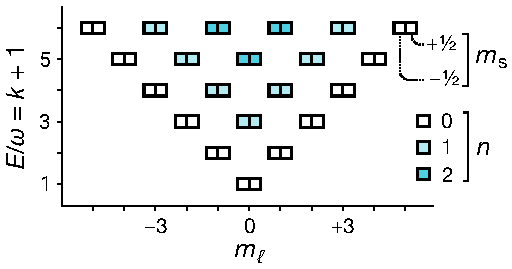
\includegraphics{fig-shell-structure-v2.pdf}
  \caption{(Color online) The 42 lowest single-particle states (the first 5 shells) in the 2D harmonic oscillator basis.  Each box represents a single-particle state arranged by $m_\ell$, $m_{\mathrm{s}}$, and energy, and the up/down arrows indicate the spin of the states.  Within each column, the principal quantum number $n$ increases as one traverses upward.}
  \label{fig:shell-structure}
\end{figure}

Single-particle states of spin-$\frac{1}{2}$ electrons also contain a spin component,
\begin{align} \label{eq:singleparticlestate}
  \langle \rho \varphi m_{\mathrm{s}}' |n m_\ell m_{\mathrm{s}}\rangle \equiv F_{n m_\ell}(\rho, \varphi) \delta_{m_{\mathrm{s}}^{} m_{\mathrm{s}}'},
\end{align}
where $m_{\mathrm{s}} = \pm\frac{1}{2}$ is the spin projection quantum number and $\delta$ is the Kronecker delta.

The energy of each single-particle state $|n m_\ell m_{\mathrm{s}}\rangle$ is given by
\begin{align} \label{eq:energysingleparticlestate}
  \varepsilon_{n m_\ell m_{\mathrm{s}}} \equiv (2 n + |m_\ell| + 1) \omega.
\end{align}
They are degenerate with respect to both spin projection $m_{\mathrm{s}}$ and \textit{shell index} $k$,
\begin{align} \label{eq:shell_index}
  k \equiv 2 n + |m_\ell|,
\end{align}
which labels each shell from zero.  The shell structure is illustrated in Fig.\ \ref{fig:shell-structure}.

Fermionic $N$-particle eigenstates of the one-body Hamiltonian $\hat{H}_1$ can be explicitly constructed as Slater determinants $|p_1 \ldots p_N\rangle$ of the single-particle states $|p_1\rangle, \ldots, |p_N\rangle$ from Eq.\ \eqref{eq:singleparticlestate}, where $|p\rangle$ is an abbreviation of $|n m_\ell m_{\mathrm{s}}\rangle$.  The Slater determinant $|p_1 \ldots p_N\rangle$ is said to \textit{occupy} the single-particle states $|p_1\rangle, \ldots, |p_N\rangle$.

When the number of particles $N$ satisfies $N = K_{\mathrm{F}} (K_{\mathrm{F}} + 1)$ for some nonnegative integer $K_{\mathrm{F}}$, there would be just enough particles to form a closed-shell Slater determinant, leading to a nondegenerate, well-isolated ground state.  The values of $N$ at which this occurs are often termed \textit{magic numbers}, and $K_{\mathrm{F}}$ is the \textit{number of filled shells} (or more abstractly the ``Fermi level'').  A single-particle state is occupied in the ground state Slater determinant if and only if $k < K_{\mathrm{F}}$, where $k$ is its shell index as defined in Eq.\ \eqref{eq:shell_index}.





\begin{figure}[h]
  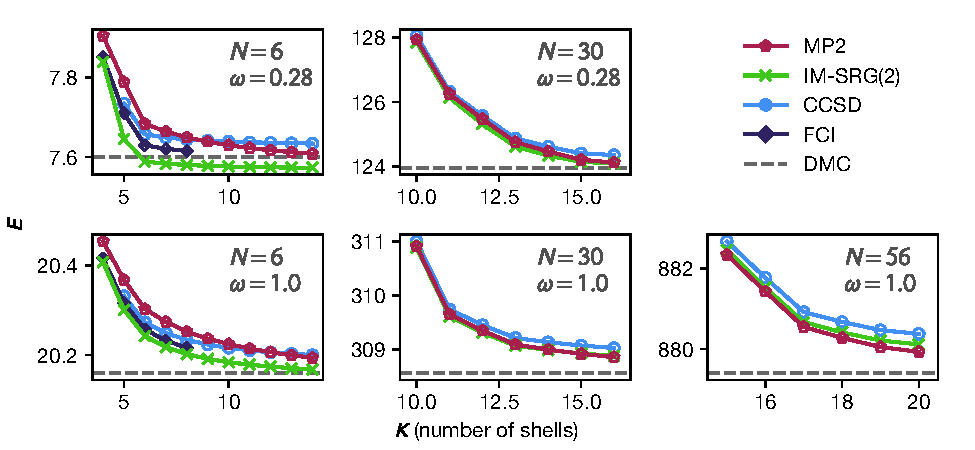
\includegraphics[width=\linewidth]{EOM/fig-gs2.pdf}
  \caption{CCD energy per electron in Hartrees for the 3D homogeneous electron gas as function of the Wigner-Seitz radius in units of Bohr radii. The calculation used periodic boundary conditions and a basis with 25 shells, resulting in a total of $1238$ single-particle states. Also plotted are the variational quantum Monte Carlo (QMC) results from \cite{LOPEZ2006}.}
  \label{fig:QDground}
\end{figure}

\begin{figure}[h]
  \centering
  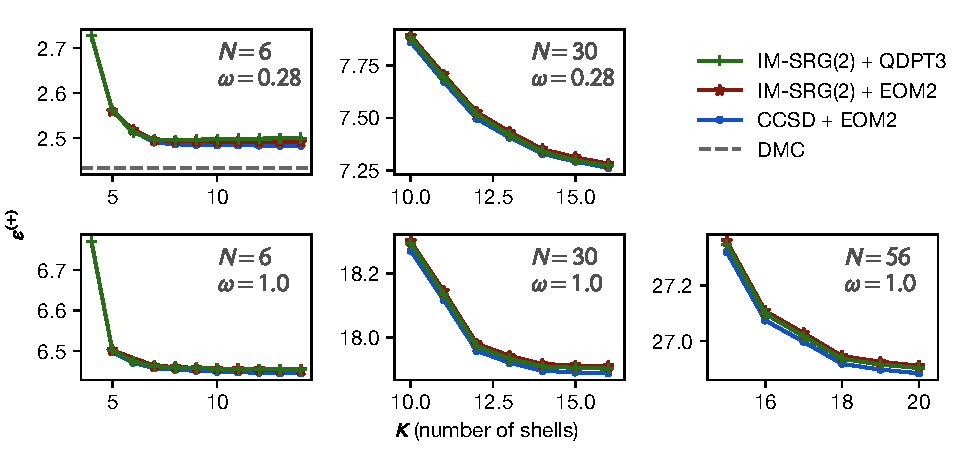
\includegraphics[\textwidth]{EOM/fig-add2.pdf}
  \caption{Progress of ab-initio nuclear structure from calculations of ground-state energies with NN+3N interactions.  Early progress was approximately linear as the problem size scaled with Moore's law while more recent progress has taken advantage of new algorithms which have outpaced Moore's law.  Data taken from \cite{HERGERTPRIVATE}.}
  \label{fig:QDadd}
\end{figure}

\begin{figure}[h]
  \centering
  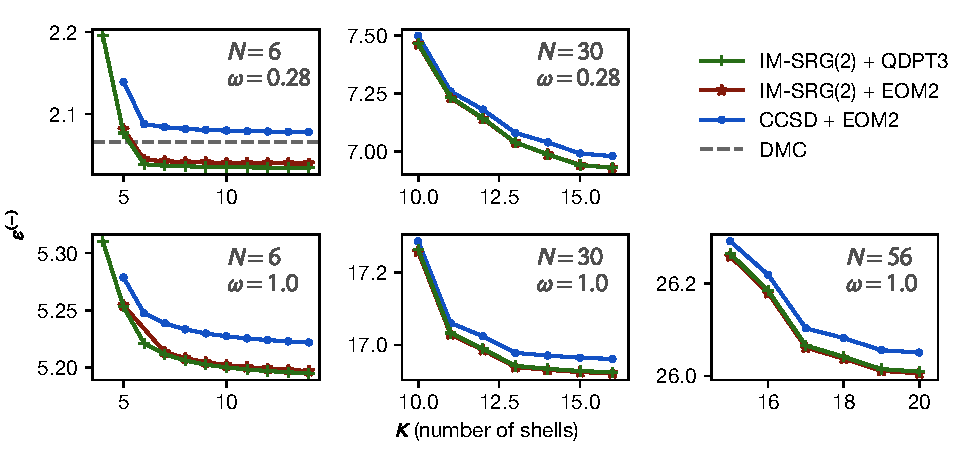
\includegraphics[\textwidth]{EOM/fig-rm2.pdf}
  \caption{Progress of ab-initio nuclear structure from calculations of ground-state energies with NN+3N interactions.  Early progress was approximately linear as the problem size scaled with Moore's law while more recent progress has taken advantage of new algorithms which have outpaced Moore's law.  Data taken from \cite{HERGERTPRIVATE}.}
  \label{fig:QDrm}
\end{figure}



\begin{figure}[h]
  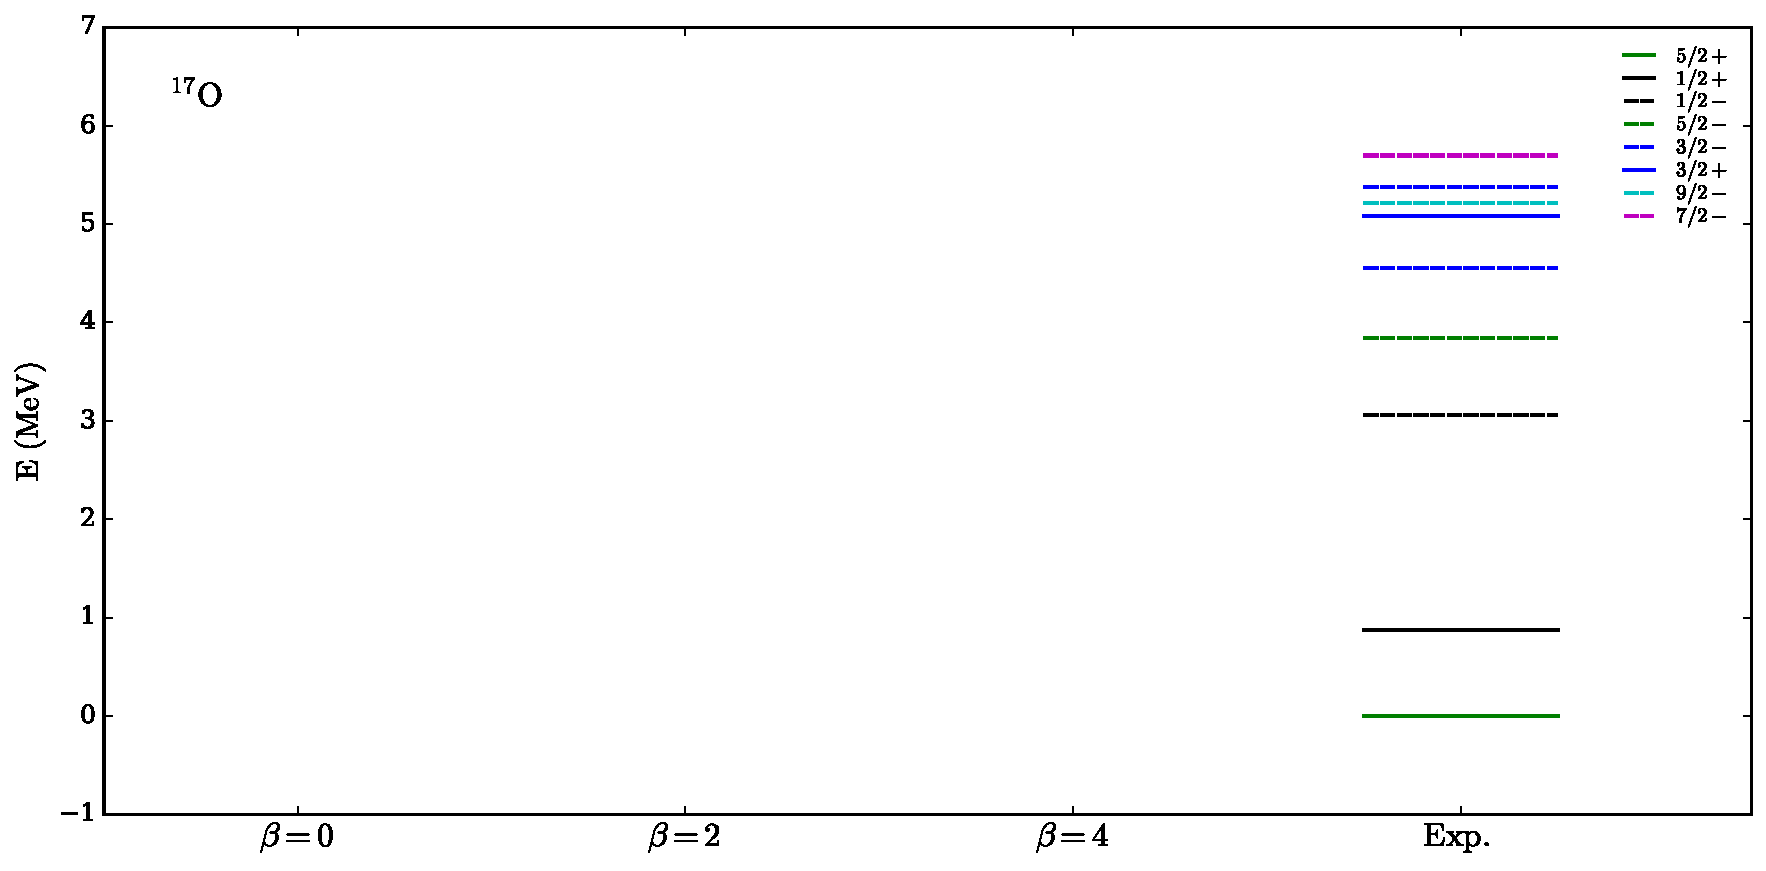
\includegraphics[width=\linewidth]{EOM/O17_PA_1.pdf}
  \caption{CCD energy per electron in Hartrees for the 3D homogeneous electron gas as function of the Wigner-Seitz radius in units of Bohr radii. The calculation used periodic boundary conditions and a basis with 25 shells, resulting in a total of $1238$ single-particle states. Also plotted are the variational quantum Monte Carlo (QMC) results from \cite{LOPEZ2006}.}
  \label{fig:QDground}
\end{figure}

\begin{figure}[h]
  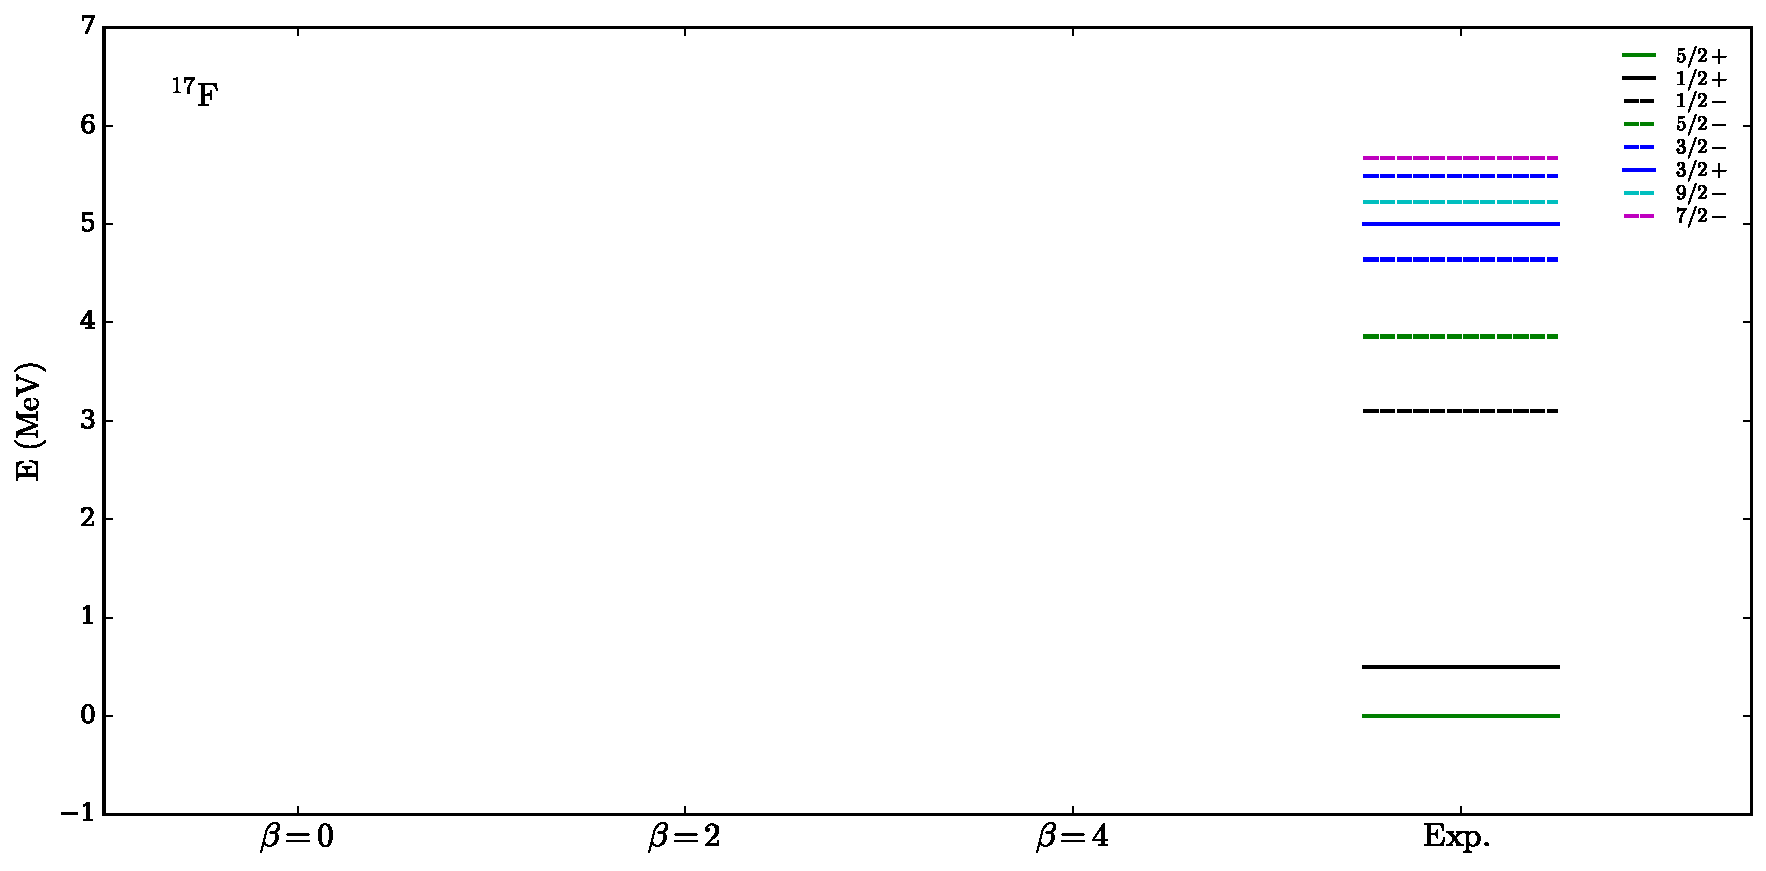
\includegraphics[width=\linewidth]{EOM/F17_PA_1.pdf}
  \caption{CCD energy per electron in Hartrees for the 3D homogeneous electron gas as function of the Wigner-Seitz radius in units of Bohr radii. The calculation used periodic boundary conditions and a basis with 25 shells, resulting in a total of $1238$ single-particle states. Also plotted are the variational quantum Monte Carlo (QMC) results from \cite{LOPEZ2006}.}
  \label{fig:QDground}
\end{figure}

\begin{figure}[h]
  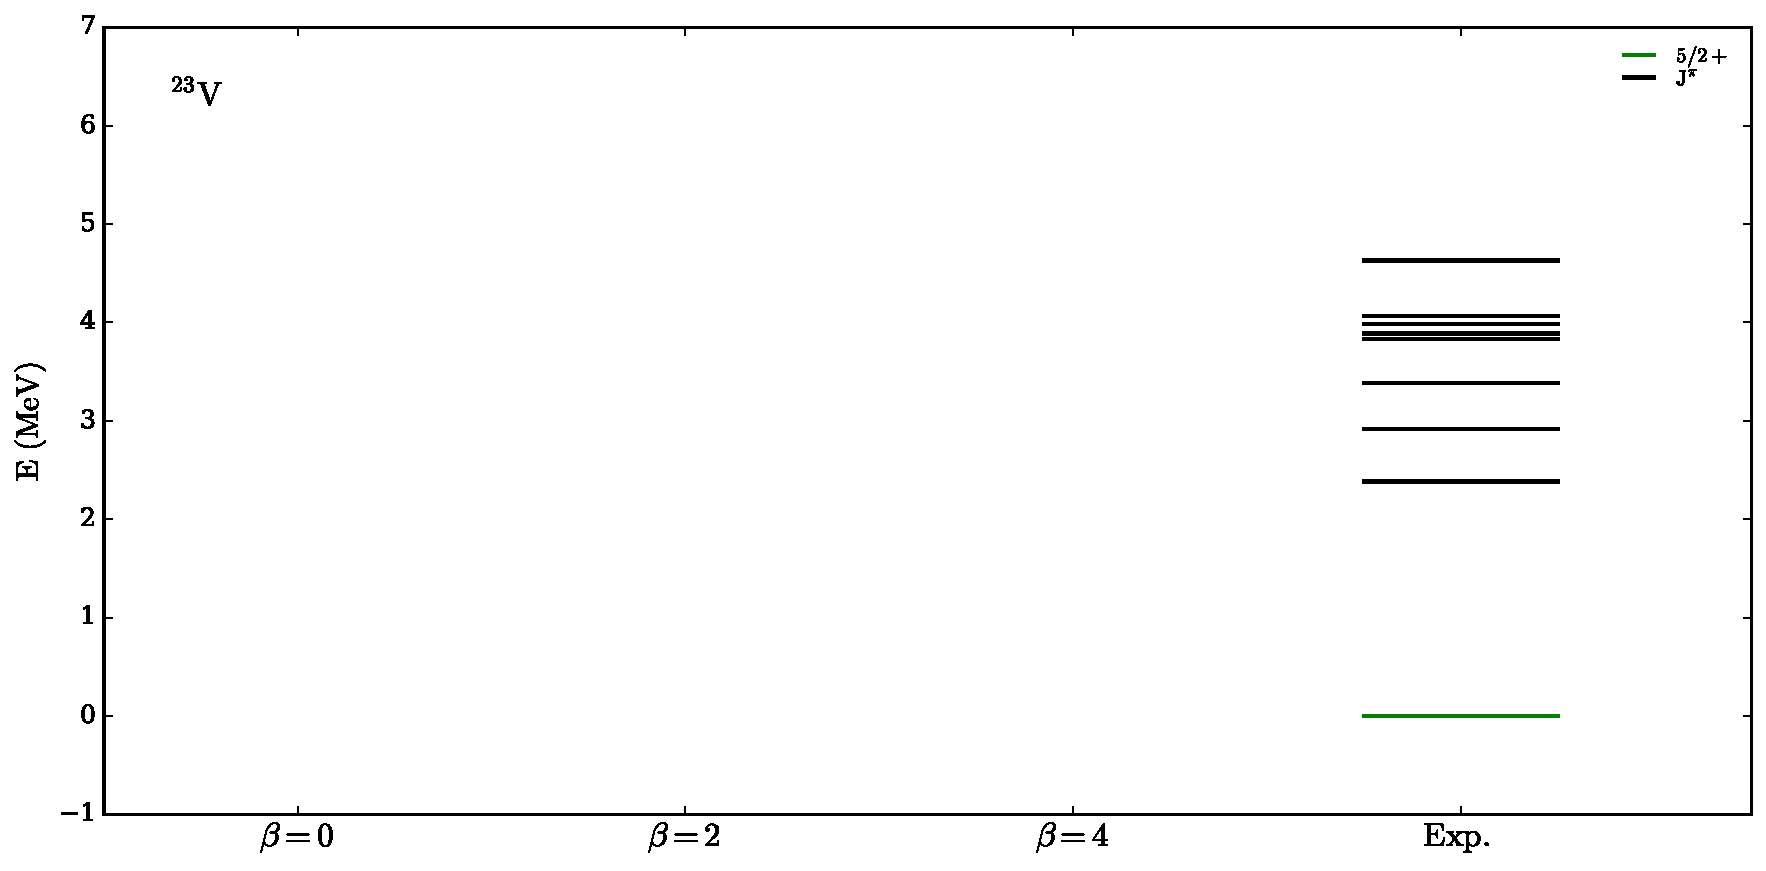
\includegraphics[width=\linewidth]{EOM/F23_PA_1.pdf}
  \caption{CCD energy per electron in Hartrees for the 3D homogeneous electron gas as function of the Wigner-Seitz radius in units of Bohr radii. The calculation used periodic boundary conditions and a basis with 25 shells, resulting in a total of $1238$ single-particle states. Also plotted are the variational quantum Monte Carlo (QMC) results from \cite{LOPEZ2006}.}
  \label{fig:QDground}
\end{figure}

\begin{figure}[h]
  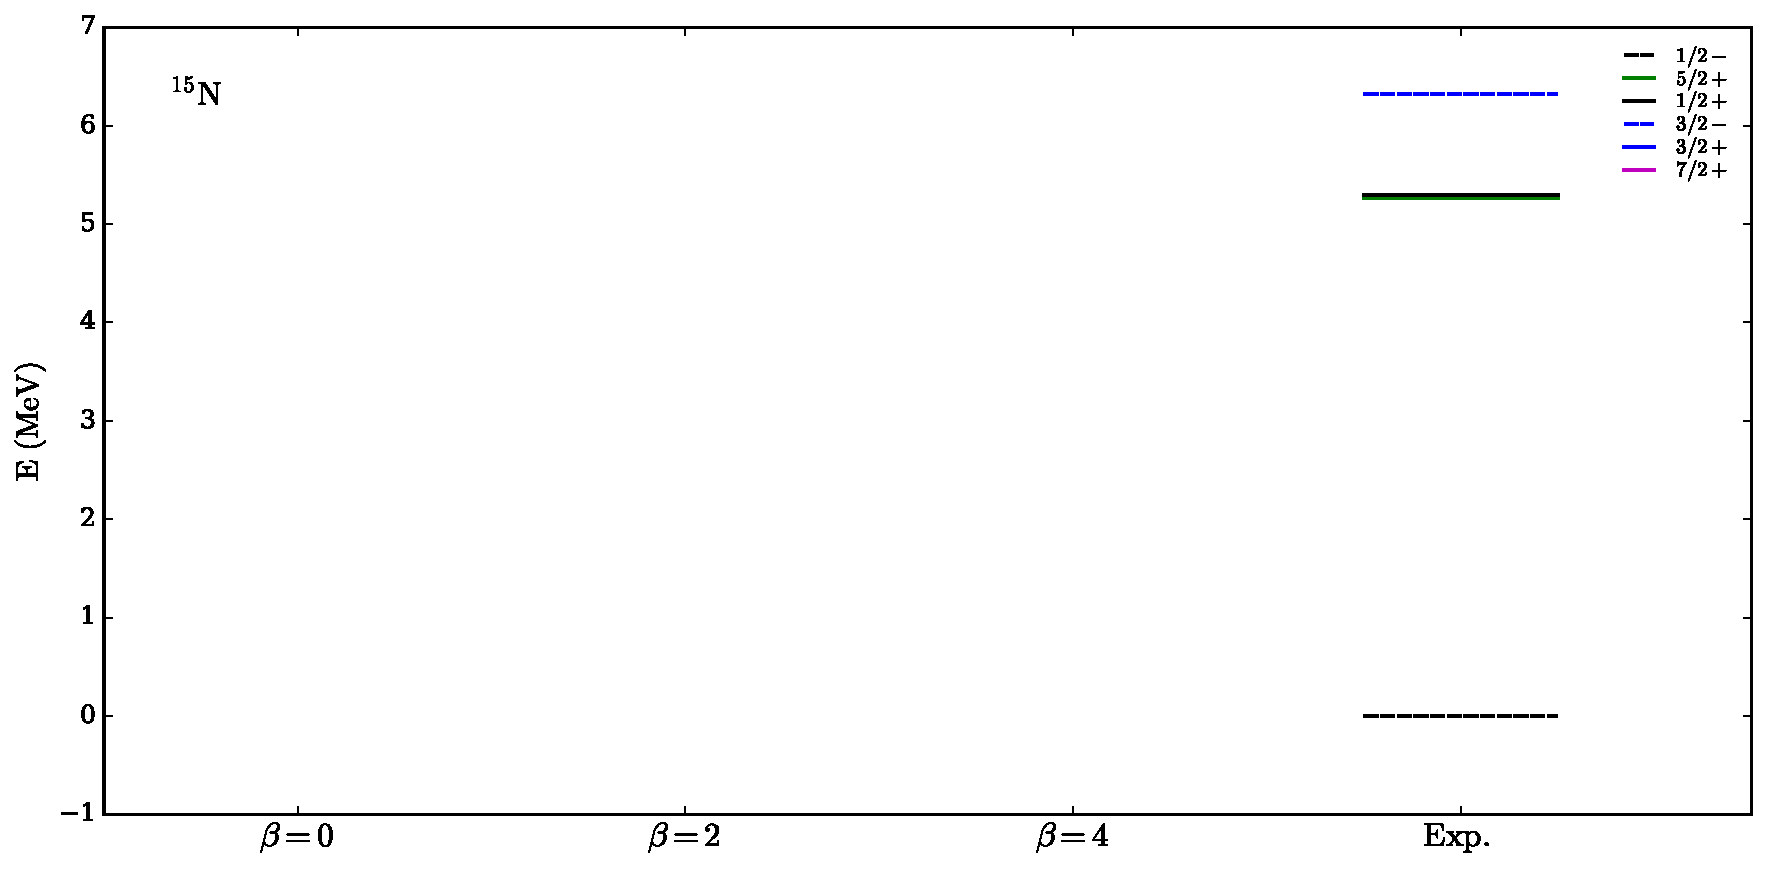
\includegraphics[width=\linewidth]{EOM/N15_PA_1.pdf}
  \caption{CCD energy per electron in Hartrees for the 3D homogeneous electron gas as function of the Wigner-Seitz radius in units of Bohr radii. The calculation used periodic boundary conditions and a basis with 25 shells, resulting in a total of $1238$ single-particle states. Also plotted are the variational quantum Monte Carlo (QMC) results from \cite{LOPEZ2006}.}
  \label{fig:QDground}
\end{figure}

\begin{figure}[h]
  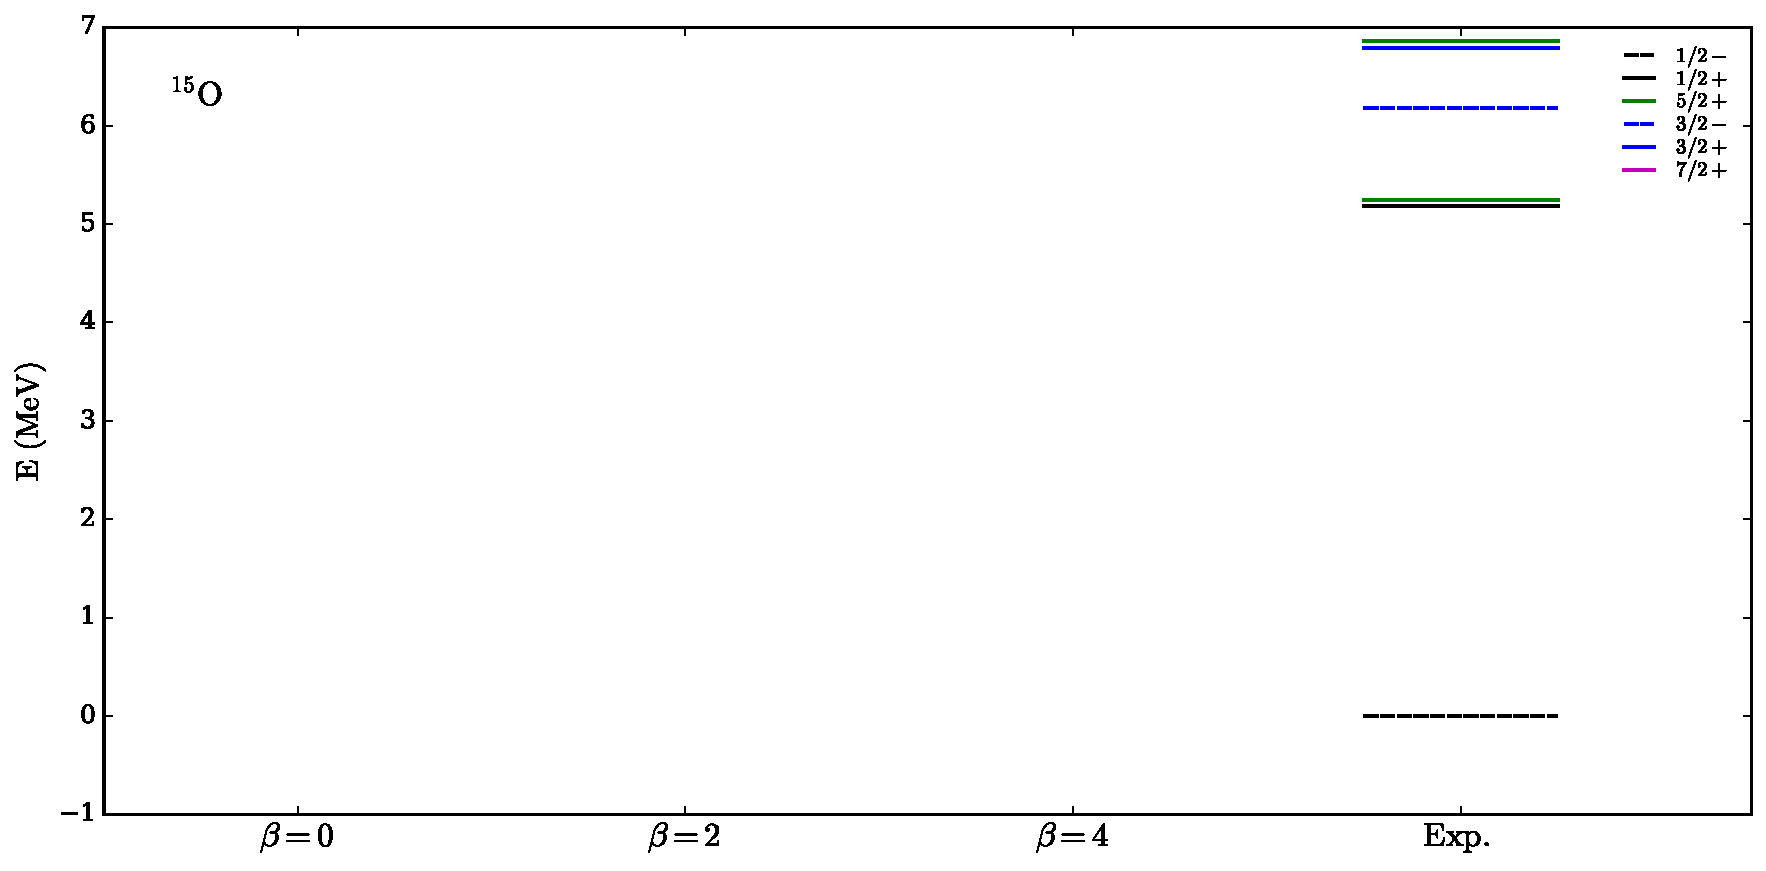
\includegraphics[width=\linewidth]{EOM/O15_PA_1.pdf}
  \caption{CCD energy per electron in Hartrees for the 3D homogeneous electron gas as function of the Wigner-Seitz radius in units of Bohr radii. The calculation used periodic boundary conditions and a basis with 25 shells, resulting in a total of $1238$ single-particle states. Also plotted are the variational quantum Monte Carlo (QMC) results from \cite{LOPEZ2006}.}
  \label{fig:QDground}
\end{figure}

\begin{figure}[h]
  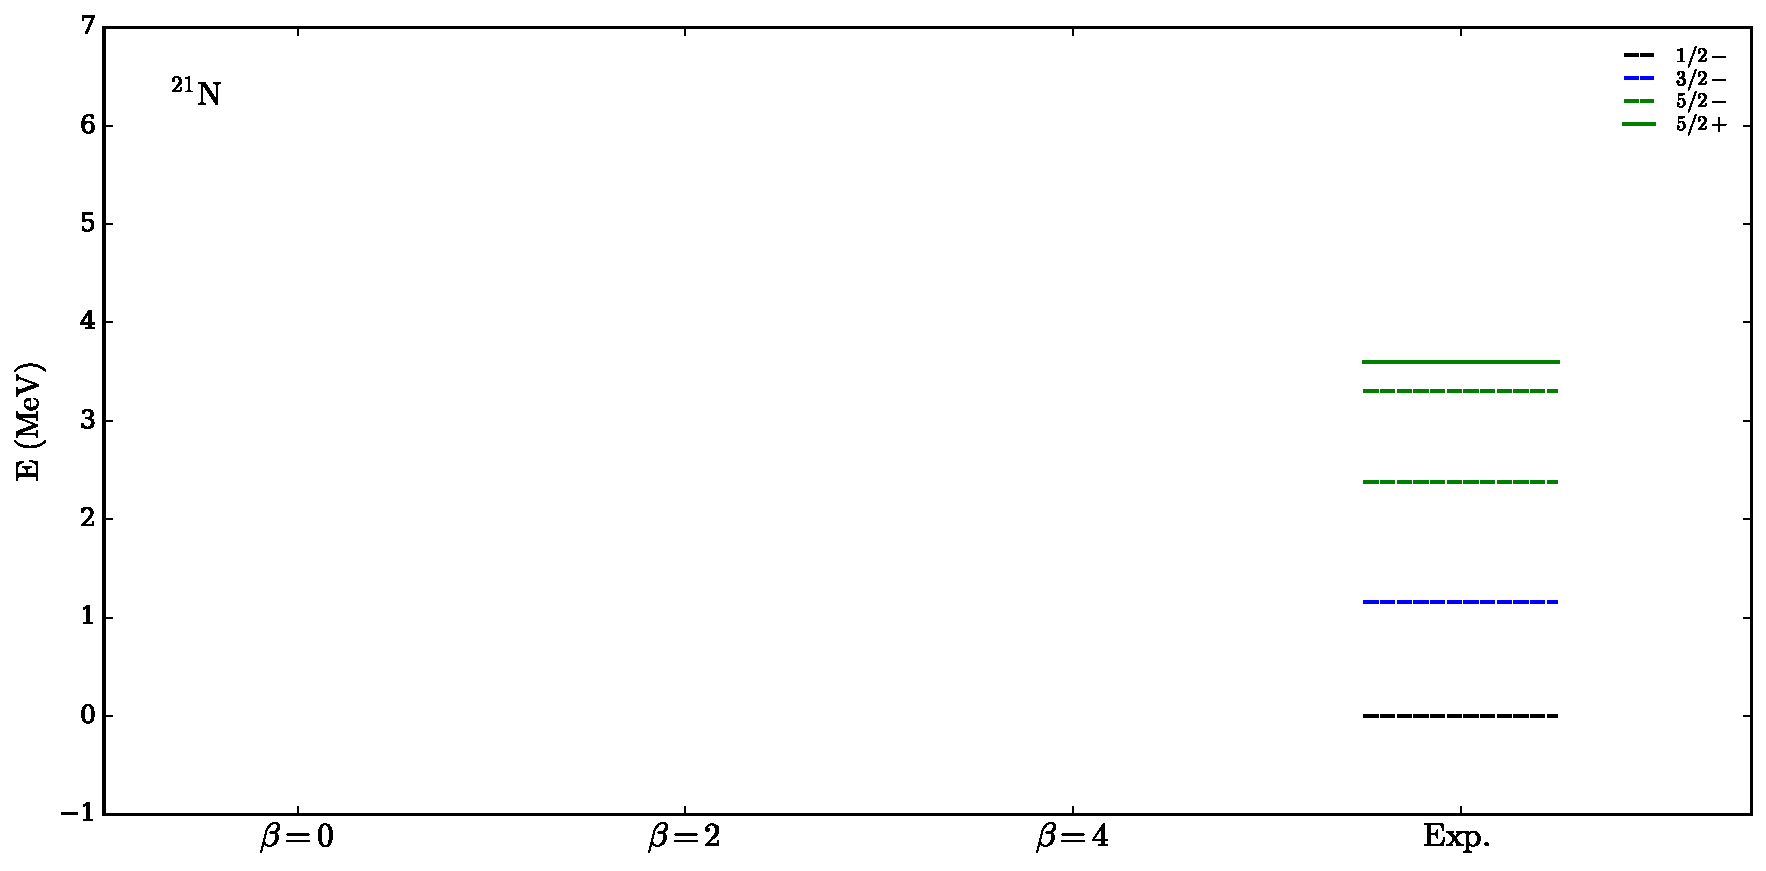
\includegraphics[width=\linewidth]{EOM/N21_PA_1.pdf}
  \caption{CCD energy per electron in Hartrees for the 3D homogeneous electron gas as function of the Wigner-Seitz radius in units of Bohr radii. The calculation used periodic boundary conditions and a basis with 25 shells, resulting in a total of $1238$ single-particle states. Also plotted are the variational quantum Monte Carlo (QMC) results from \cite{LOPEZ2006}.}
  \label{fig:QDground}
\end{figure}

\begin{figure}[h]
  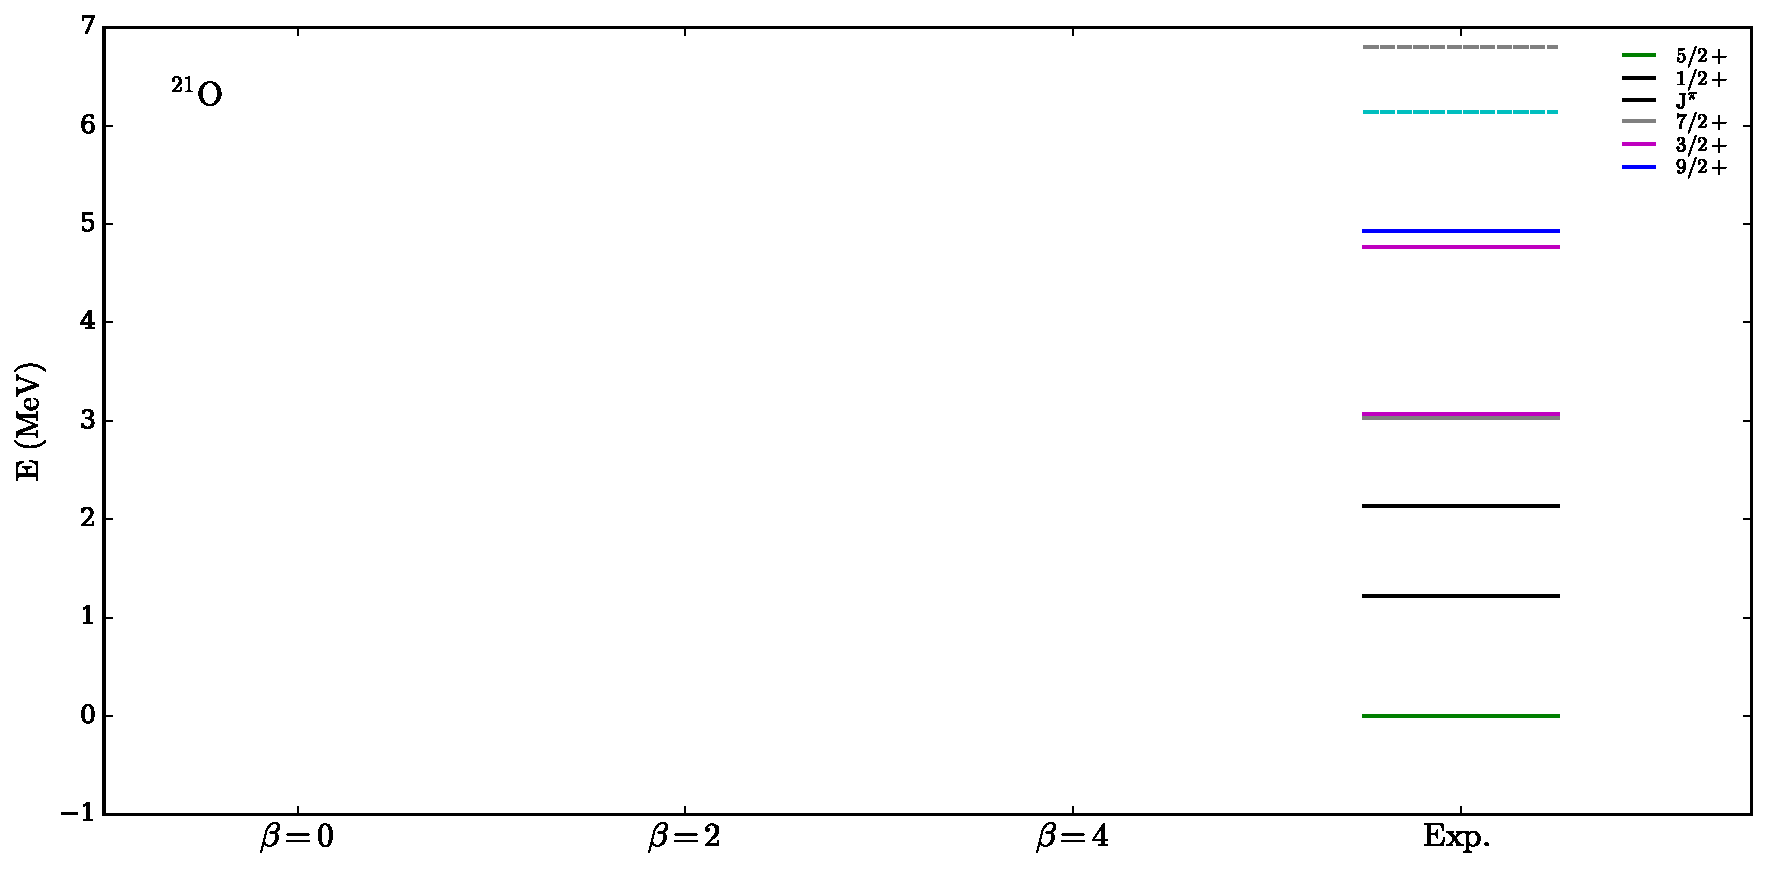
\includegraphics[width=\linewidth]{EOM/O21_PA_1.pdf}
  \caption{CCD energy per electron in Hartrees for the 3D homogeneous electron gas as function of the Wigner-Seitz radius in units of Bohr radii. The calculation used periodic boundary conditions and a basis with 25 shells, resulting in a total of $1238$ single-particle states. Also plotted are the variational quantum Monte Carlo (QMC) results from \cite{LOPEZ2006}.}
  \label{fig:QDground}
\end{figure}

\end{document}
